\documentclass[a4paper,12pt,oneside]{article}
\usepackage{graphicx}
\usepackage{hyperref}
\usepackage[T1]{fontenc}
\usepackage[utf8]{inputenc}
\usepackage{setspace}
\usepackage{amsmath}
\usepackage{amssymb}

\begin{document}

    \thispagestyle{plain}
    \begin{center}
        \normalsize
        \textbf{Assignment 1}
            
        \vspace{0.2cm}
        \normalsize
        19/10/2022
            
        \vspace{0.2cm}
        \textbf{Francesco Refolli 865955}
    \end{center}

    \section{Esercizio 1}

    \begin{align}
        \text{$max \; x_1 + x_2$} \\
        \text{$x_1 + x_2 \leq 2$} \\
        \text{$2 x_1 - x_2 \leq 0$} \\
        \text{$x_1, x_2 \geq 0$}
    \end{align}

    Costruisco il grafico con le equazioni dei vincoli lungo l'asse $x_1 \times x_2$.
    Riscrivo per comodita' i primi due vincoli in forma equivalente:

    \begin{align}
        \text{$x_1 \leq 2 - x_2$} \\
        \text{$x_1 \leq \frac {x_2} 2$}
    \end{align}

    \begin{center}
        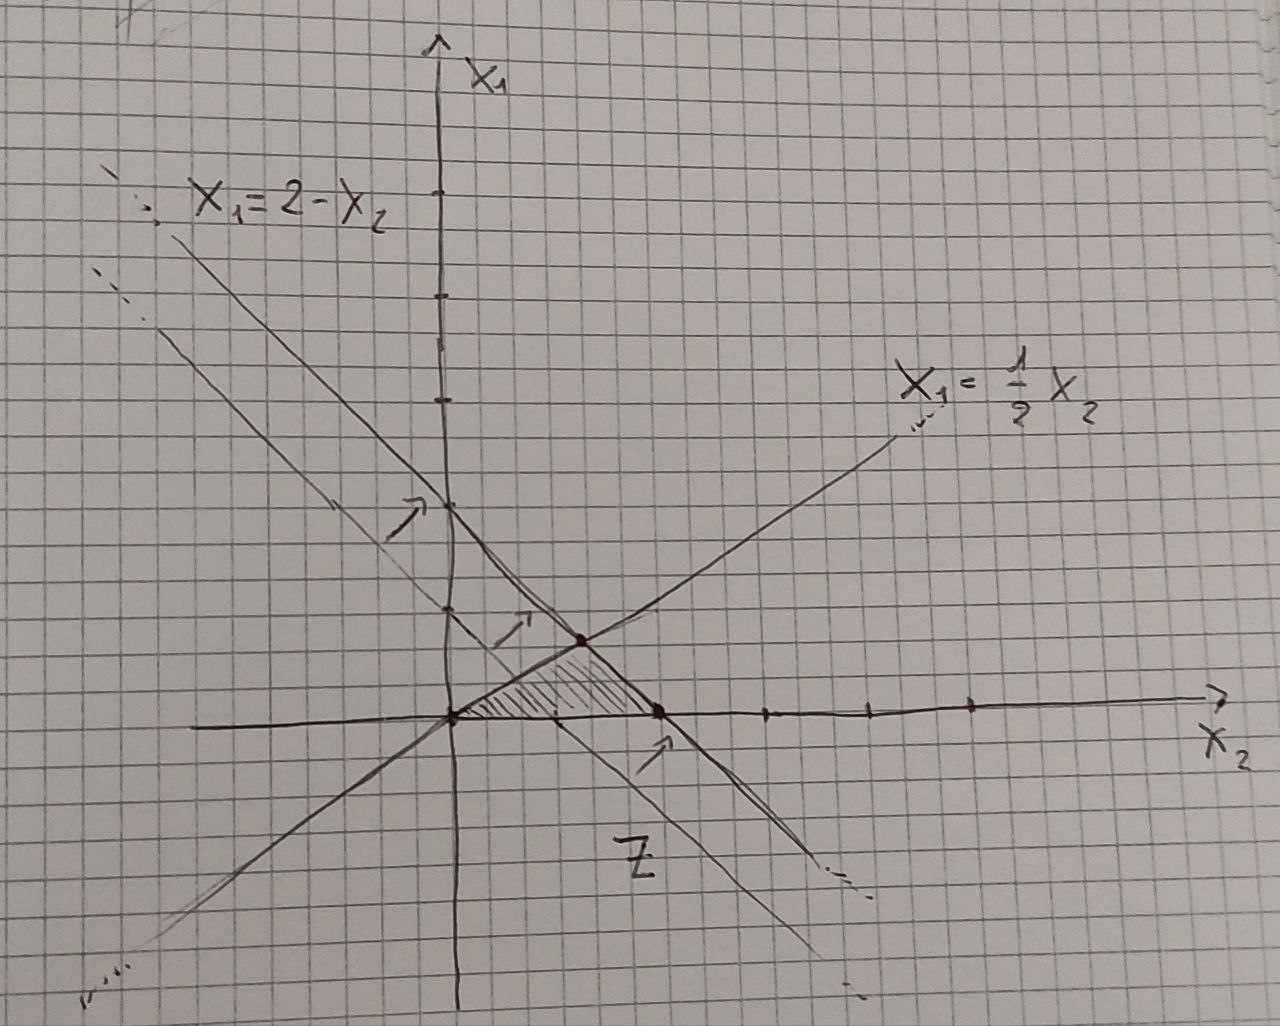
\includegraphics[width=12cm]{grafico.jpg}
    \end{center}

    Il vetto del gradiente della funzione obiettivo $g$ = <$1, 1$> , composto dalle derivate parziali delle componenti della funzione obiettivo, e' perpedincolare al vincolo $x_1 \leq 2 - x_2$, quindi il problema ha \textbf{Infinite Soluzioni Ottime}. \\*
    Le soluzioni sono tutte le coppie <$x_1, x_2$> che risiedono nello spigolo della regione obiettivo su cui si poggia il vincolo $x_1 \leq 2 - x_2$. Ovvero tutti i punti sul segmento delimitato dai punti: ($0, 2$),  ($\frac 2 3, \frac 4 3$).

    \section{Esercizio 2}

    \begin{align}
        \text{$max \; x_1 + x_2$} \\
        \text{$x_1 + x_2 - x_3 = 2$} \\
        \text{$2 x_1 - x_2 \leq 0$} \\
        \text{$x_1, x_2 \geq 0$} \\
        \text{$x_3 \leq 0$}
    \end{align}

    \paragraph{Conversione in forma aumentata}

    \subparagraph{1}

    La forma aumentata non prevede vincoli di non positivita', quindi inverto il segno di $x_3$ in tutti i vincoli:

    \begin{align}
        \text{$max \; x_1 + x_2$} \\
        \text{$x_1 + x_2 + x_3 = 2$} \\
        \text{$2 x_1 - x_2 \leq 0$} \\
        \text{$x_1, x_2, x_3 \geq 0$}
    \end{align}

    \subparagraph{2}

    Aggiungo una variabile di slack $x_4$ per portare il vincolo $\leq$ in vincolo $=$.

    \begin{align}
        \text{$max \; x_1 + x_2$} \\
        \text{$x_1 + x_2 + x_3 = 2$} \\
        \text{$2 x_1 - x_2 + x_4 = 0$} \\
        \text{$x_1, x_2, x_3, x_4 \geq 0$}
    \end{align}

    \subparagraph{3}

    Quindi esporto la funzione obiettivo $f(x)$ in un vincolo $Z - f(x) = 0$.

    \begin{align}
        \text{$max \; Z$} \\
        \text{$Z - x_1 - x_2 = 0$} \\
        \text{$x_1 + x_2 + x_3 = 2$} \\
        \text{$2 x_1 - x_2 + x_4 = 0$} \\
        \text{$x_1, x_2, x_3, x_4 \geq 0$}
     \end{align}

    \paragraph{Risoluzione con tableau}
   
    \begin{center}
        \begin{tabular}{|c|c|c|c|c|c|}
            \hline
            Z & $x_1$ & $x_2$ & $x_3$ & $x_4$ & b\\
            \hline
            1 & -1 & -1 & 0 & 0 & 0\\
            0 & 1 & 1 & 1 & 0 & 2\\
            0 & 2 & -1 & 0 & 1 & 0\\
            \hline
        \end{tabular}
    \end{center}
    \paragraph{iteration 1}
    Scelgo la colonna 1 perche' non esiste un coefficiente in prima riga negativo piu' basso. \\
    Scelgo la riga 2 che ha il rapporto minimo. \\
    Ricalcolo la tabella.
    Questo ha l'effetto di scambiare $x_2$ della base con $x_1$. \
    \begin{center}
        \begin{tabular}{|c|c|c|c|c|c|}
            \hline
            Z & $x_1$ & $x_2$ & $x_3$ & $x_4$ & b\\
            \hline
            1.0 & 0.0 & -$\frac 3 2$ & 0.0 & $\frac 1 2$ & 0.0\\
            0.0 & 0.0 & $\frac 3 2$ & 1.0 & -$\frac 1 2$ & 2.0\\
            0.0 & 1.0 & -$\frac 1 2$ & 0.0 & $\frac 1 2$ & 0.0\\
            \hline
        \end{tabular}
    \end{center}
    \paragraph{iteration 2}
    Scelgo la colonna 2 perche' non esiste un coefficiente in prima riga negativo piu' basso. \\
    Scelgo la riga 1 che ha il rapporto minimo. \\
    Ricalcolo la tabella.
    Questo ha l'effetto di scambiare $x_1$ della base con $x_2$. \
    \begin{center}
        \begin{tabular}{|c|c|c|c|c|c|}
            \hline
            Z & $x_1$ & $x_2$ & $x_3$ & $x_4$ & b\\
            \hline
            1.0 & 0.0 & 0.0 & 1.0 & 0.0 & 2.0\\
            0.0 & 0.0 & 1.0 & $\frac 2 3$ & -$\frac 1 3$ & $\frac 4 3$\\
            0.0 & 1.0 & 0.0 & $\frac 1 3$ & $\frac 1 3$ & $\frac 2 3$\\
            \hline
        \end{tabular}
    \end{center}
    \paragraph{iteration 3}
    La prima riga non contiene piu' valori negativi, l'algoritmo del simplesso si arresta. \\
    La soluzione di base corrente e' <$x_1$,$x_2$,$x_3$,$x_4$> = <$\frac 2 3$,$\frac 4 3$,0,0>\*
    Quindi una soluzione al problema PL e' <$x_1$,$x_2$> = <$\frac 2 3$,$\frac 4 3$>\*
\end{document}
